\section{El-ovn}
Rockwool besluttet i desember 2018 å investere i en ny smelteovn som vil benytte elektrisitet som energikilde. Beslutningen ble tatt etter å ha fått godkjent søknaden om 101,5 millioner kroner i støtte fra Enova. Enova er forvalter av Energifondet, og støtter norske bedrifter som ønsker en omstilling til lavutslippssamfunnet \cite{enova}. En elektrisk smelteovn er ikke tilgjengelig i markedet i dag, og investeringen krever at Rockwool selv utvikler nye og hensiktsmessige teknologiske løsninger tilpasset egen produksjon. Beregninger foretatt av selskapet viser til et investeringsbeløp på ca. 340 millioner kroner som fordeles i 2018, 2019 og 2020. Beløpet gjelder investeringer i innovasjon, teknologi og personalopplæring. 

\indent \newline
En el-ovn forventes å håndtere opp til 40\% gammel steinull (resirkulering), med en kapasitet på rundt 11.000 tonn steinullavfall fra byggeplasser. Dette tilsvarer mer enn totalt deponi av steinull per år fra byggmarkedet. Norge er i en særstilling når det gjelder avfall, hvor avfall til deponi, både fra produksjon og byggeplass, har vært relativt billig i flere år. Situasjonen er imidlertid i ferd med å endre seg da nye markeds- og myndighetskrav forventes fremover. Avfallet fra produksjonen representerer stangmøllemel (granulert ull) og små mengder avfall/kapp av ny isolasjon som returneres fra markedet. Øvrig produksjonsavfall består av ovnsbunn (jern, slagger og fines) og flyveaske. Teknologien vil kunne føre til en avfallsreduksjon på 19.677 tonn per år. Det tilsvarer en reduksjon på ca. 95\% sammenlignet med 2017.

\begin{table}[H]
  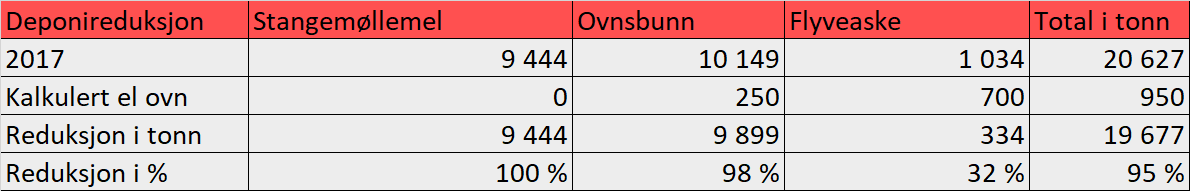
\includegraphics[width=\linewidth]{tabeller/deponireduksjon.png}
  \caption{Deponireduksjon}
  \label{tbl:deponireduksjon}
\end{table}

\indent \newline
Konvertering fra koks til elektrisitet vil også føre til store endringer med tanke på CO2-utslippet. Analyser fra Rockwool viser til en potensiell reduksjon i CO2-nivå med omtrent 80\%. Investeringen vil dermed føre til reduserte kostnader i forbindelse med CO2-kvoter, deponi og resirkulering. 

\begin{table}[H]
  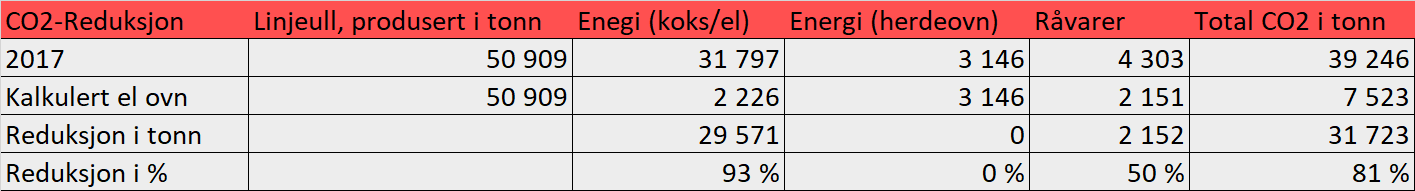
\includegraphics[width=\linewidth]{tabeller/co2reduksjon.png}
  \caption{CO2-reduksjon}
  \label{tbl:co2reduksjon}
\end{table}

\indent \newline
Investeringen baserer seg på utvikling innenfor teknologi og innovasjon i fire hovedelementer;

\begin{itemize}
\item[1.] Sikkerhet - Bygge den hittil største Submerged Arc Furnace (SAF) med lite smelteblad. En normal SAF-ovn med ønsket charge rate på 11,5 tonn per time vil ha en diameter på 8-9 meter og holde 189 tonn smelte. For å redusere risiko skal denne reduseres ned til 5,5-6 meter og holde 73 tonn smelte. Dette innebærer at en ny ovnstype med høyere “loadfaktor” må utvikles, noe som gir en høyere termisk belastning på ovnen og oppmuringsmaterialer.

\item[2.] Utvikle en SAF som kan håndtere en høy last samtidig med høy resirkuleringsandel. Dagens el-ovner har en begrensning i load og resirkuleringsfaktor, det vil si enten en høy load og lav resirkulering eller lav load og høy resirkulering. En resirkuleringsandel på 40\% vil stille nye krav til røykgassrensning. Resirkulert steinull inneholder mer organisk materiale sammenlignet med kun bruk av stein som råvare. Mengden rørgasser forventes derfor å øke sammenlignet med dagens produksjon.

\item[3.] Temperaturstabilitet - Utvikle en ny homogeniseringskanal.Fra ovn til spinnemaskiner er det over tre meter. Det ligger utfordringer i å sikre en stabil smeltetemperatur til spinnemaskinene. Det må derfor utvikles en homogeniseringskanal mellom ovn og eksisterende spinnere, da en slik kanal ikke er tilgjengelig i dag. Ved å sikre en stabil temperatur på +/- 10 grader celcius vil kanalen resultere i et høyere spinneutbytte.

\item[4.] Utvikle rett sammensetning av lining og effektivisere liningsbyttet. En høy grad av resirkulering vil stille nye krav til isolasjonsmateriale på innsiden av ovnen (lining). En ingeniørgruppe i Rockwool arbeider med å utvikle den rette sammensetningen for riktig lining. Erfaring viser at resirkulering øker slitasjen på liningen. Dette vil påvirke vedlikeholdsintervallene ved å gå fra hvert tredje år til hvert andre år. Målet er å redusere tiden det tar å skifte lining fra 3-4 uker til under 2 uker.
\end{itemize}

\indent \newline
I forbindelse med dimensjoneringen av smelteovnen vil selskapet produsere i et kapasitetsområde som ikke er prøvd ut tidligere. Overdimensjoneringen vil øke investeringen og risikoen i prosjektet, men anses som nødvendig for å opprettholde produksjonskapasiteten i Moss. Hvis temperaturstabillitet ikke oppnås, kan avfallsprosenten stige eksplosivt til 10-15\%. En marginal endring på 1\% resulterer i økte kostnader på 1,2 millioner kroner. Dette er isolert sett den største risikoen i prosjektet.

\indent \newline
I tillegg påløper det risiko knyttet til drift i form av en situasjon hvor det ikke oppnås full effekt. Dette fører til at resten av produksjonsanlegget ikke anvendes optimalt i forhold til produksjonsvolumene det er tilpasset til. Det vil også med stor sannsynlighet oppstå hyppigere og lengre stopp i produksjon, spesielt med tanke på liningslitasje. 

\section{Nåværende smelteteknologi}
Smelteteknologien som blir brukt i dag er en kupolovn, hvor energibærerne hovedsakelig består av koks og kalsinert karbon. Råvarer som benyttes er Anortositt, Gabbro, Fundia slagg, Dolomitt og Merox slagg. Per i dag har ikke kupolovnen nødvendig teknologi til å håndtere avfall fra byggeplasser.

\indent \newline
Å basere produksjonen hovedsakelig på fossile energibærere kan være risikofullt og kostbart, da markedsutviklingen går mot grønnere produkter. Klimarisikoen kommer til syne på et overordnet nivå, i form av Paris-avtalen og FNs bærekraftsmål, og på et underordnet nivå, i form av krav fra byggherrer og entreprenører. Rockwool har allerede erfart dette ved at byggaktørene har begynt å velge produkter som har et lavere CO2-avtrykk. Dette er gitt at øvrige byggetekniske krav er ivaretatt og prisen er konkurransedyktig. 

\indent \newline
Fokus på sirkulær økonomi har også fått større betydning de senere årene. Byggavfall er en stor kilde til avfall, og det forventes at markedet på sikt vil stille strengere krav til materialgjenvinning. I følge Erik Ølstad har eksempelvis Statsbygg signalisert at Rockwool må forberede seg på å endre dagens praksis og være i stand til å ta i mot retur av steinullavfall i fremtiden. 

\section{Brun smelteteknologi (BAT)}
En alternativ investering er en IMF-ovn (fluid bed ovn) hvor energibæreren er kull eller gass. Dette er en BAT-løsning (Best Available Technology) som kan bli gjennomført basert på Rockwool-konsernets egen smelteteknologi. Investeringen ligger på ca. 5 millioner kroner og innebærer redusert ovnsbunn og installasjon av full innvendig lining. Kostnaden for en slik smeltelinje ligger på samme nivå som en elektrisk smeltelinje. Imidlertid vil en BAT-oppdatering maksimalt resultere i 20-30\% CO2-reduksjon. Dette er derfor ikke en bærekraftig investering med en 10-års horisont. Høye vedlikeholdskostnader vil i tillegg gjøre det vanskelig for Rockwool å finansiere en slik løsning, da kapasiteten i Moss ikke er stor nok. I følge Rockwool var dette ikke et reelt alternativ, og beslutningen stod mellom å investere i el-teknologi eller å fortsette med nåværende teknologi. Vi vil på bakgrunn av dette ikke gå videre med å undersøke lønnsomheten av dette alternativet.
